\documentclass[aspectratio=169]{beamer}

\usetheme{Madrid}
\usecolortheme{seahorse}
\setbeamertemplate{navigation symbols}{}
\setbeamertemplate{footline}[frame number]
\setbeamertemplate{bibliography item}{\insertbiblabel}

\usepackage[T1]{fontenc}
\usepackage{amsmath}
\usepackage{booktabs}
\usepackage{graphicx}
\usepackage{hyperref}
\usepackage{tikz}
\usetikzlibrary{arrows.meta,calc,positioning,shapes.geometric}

\title[Inference vs Retrieval]{Inference vs Retrieval\\for Multimodal Garbage Classification}
\subtitle{Evaluating Traditional Models and Novel DNDS Heuristics}
\author{Maheen Hoque \and Arman Hossain Dipu Khan \and Lila Sanjay Kumar Gorlie}
\institute{University of Calgary}
\date{April 2026}

\begin{document}

\begin{frame}
  \titlepage
\end{frame}

\begin{frame}{Outline}
  \tableofcontents
\end{frame}

\section{Motivation}
\begin{frame}{Problem Motivation}
\begin{itemize}
  \item Automated sorting benefits from multimodal image+text signals \cite{alexakis2025enhanced}.
  \item Supervised pipelines degrade under imbalance and shift \cite{islam2026learning}.
  \item RAC uses neighbor evidence at inference time \cite{li2024kra}.
  \item \textbf{DNDS} reweights RAC scores by class density to reduce majority bias.
\end{itemize}
\end{frame}

\begin{frame}{Research Questions}
\begin{enumerate}
  \item Does DNDS beat traditional multimodal inference?
  \item Is DNDS robust under severe imbalance?
  \item Does DNDS improve as database size grows?
  \item Which DNDS variant is best overall?
\end{enumerate}
\vspace{4pt}
\textbf{Dataset:} 16,957 samples across 4 classes (Black, Blue, Green, TTR) \cite{cazarin2025garbage}.
\end{frame}

\section{Data and Methods}
\begin{frame}{Dataset and Class Imbalance}
\begin{itemize}
  \item Black: 3459
  \item Blue: 6720
  \item Green: 3492
  \item TTR: 3286
  \item Blue is about 1.9x larger than minority classes.
  \item Class skew can bias both decision boundaries and retrieval votes.
\end{itemize}
\vspace{2pt}
{\scriptsize Dataset source: \cite{cazarin2025garbage}.}
\end{frame}

\begin{frame}{Dataset and Class Imbalance: Distribution}
\centering
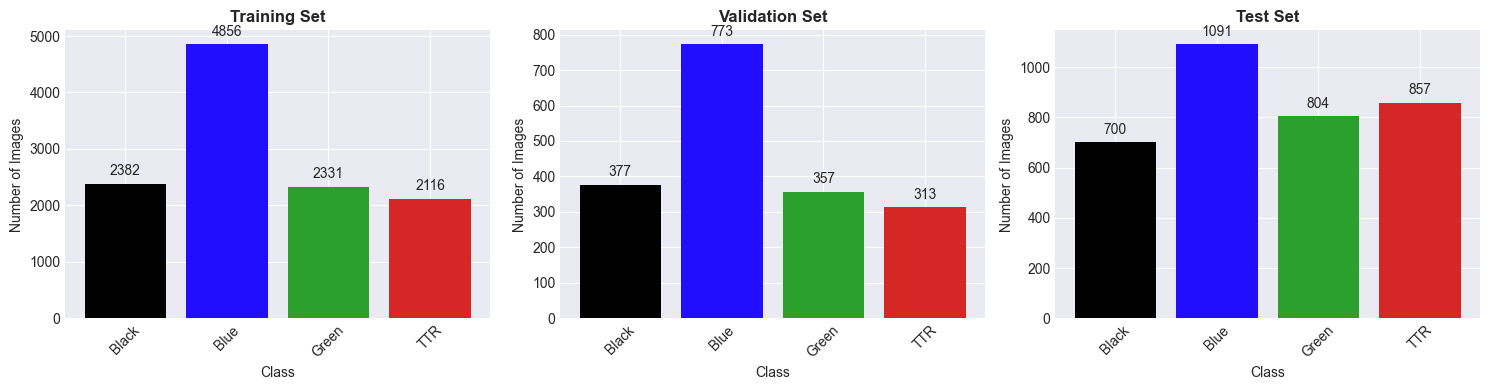
\includegraphics[width=0.9\linewidth,height=0.75\textheight,keepaspectratio]{images/trash_dataset.png}
\\[-2pt]
{\scriptsize Class distribution used in this study.}
\end{frame}

\begin{frame}{Method Overview: Traditional vs RAC}
\centering
\scriptsize
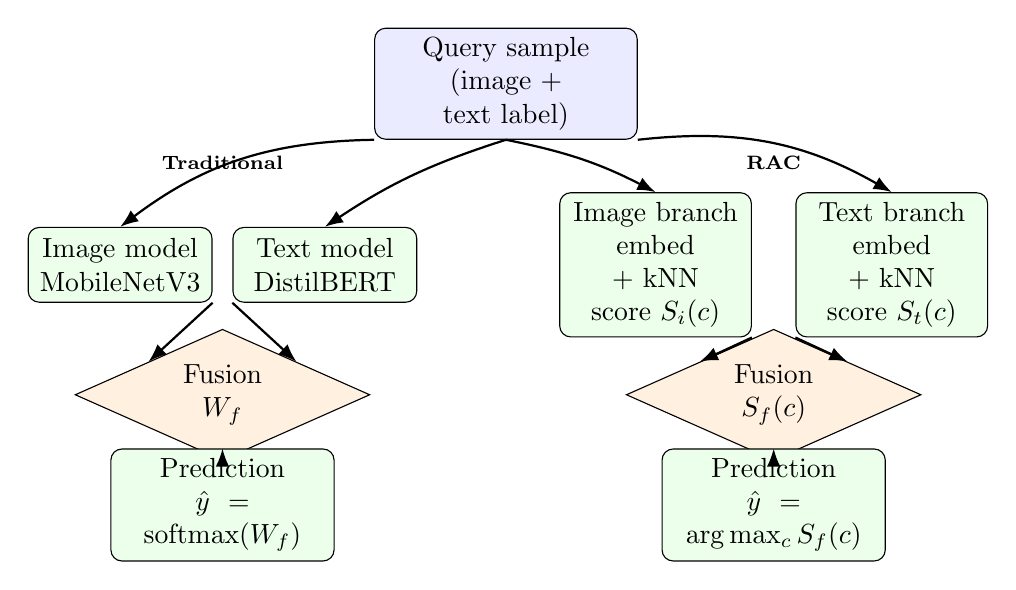
\begin{tikzpicture}[
  querybox/.style={draw, rounded corners, align=center, text width=3.1cm, minimum height=0.9cm, fill=blue!8},
  modelbox/.style={draw, rounded corners, align=center, text width=2.1cm, minimum height=0.95cm, fill=green!8},
  branchbox/.style={draw, rounded corners, align=center, text width=2.2cm, minimum height=1.05cm, fill=green!8},
  predbox/.style={draw, rounded corners, align=center, text width=2.6cm, minimum height=0.95cm, fill=green!8},
  diamondbox/.style={draw, diamond, aspect=2.25, align=center, inner sep=1pt, text width=1.8cm, minimum height=0.95cm, fill=orange!12},
  labelbox/.style={font=\bfseries\scriptsize},
  arrow/.style={-Latex, thick}
]

\node[querybox] (input) at (0,0) {Query sample\\(image + text label)};

\node[labelbox] at (-3.6,-1.0) {Traditional};
\node[modelbox] (imgModel) at (-4.9,-2.3) {Image model\\MobileNetV3};
\node[modelbox] (txtModel) at (-2.3,-2.3) {Text model\\DistilBERT};
\node[diamondbox] (tradFuse) at (-3.6,-3.95) {Fusion\\$W_f$};
\node[predbox] (predTrad) at (-3.6,-5.35) {Prediction\\$\hat y=\mathrm{softmax}(W_f)$};

\node[labelbox] at (3.4,-1.0) {RAC};
\node[branchbox] (imgRac) at (1.9,-2.3) {Image branch\\embed + kNN\\score $S_i(c)$};
\node[branchbox] (txtRac) at (4.9,-2.3) {Text branch\\embed + kNN\\score $S_t(c)$};
\node[diamondbox] (racFuse) at (3.4,-3.95) {Fusion\\$S_f(c)$};
\node[predbox] (predRac) at (3.4,-5.35) {Prediction\\$\hat y=\arg\max_c S_f(c)$};

\draw[arrow] (input.south west) to[bend right=18] (imgModel.north);
\draw[arrow] (input.south) to[bend right=8] (txtModel.north);
\draw[arrow] (imgModel.south east) -- (tradFuse.north west);
\draw[arrow] (txtModel.south west) -- (tradFuse.north east);
\draw[arrow] (tradFuse) -- (predTrad);

\draw[arrow] (input.south) to[bend left=8] (imgRac.north);
\draw[arrow] (input.south east) to[bend left=18] (txtRac.north);
\draw[arrow] (imgRac.south east) -- (racFuse.north west);
\draw[arrow] (txtRac.south west) -- (racFuse.north east);
\draw[arrow] (racFuse) -- (predRac);
\end{tikzpicture}
\end{frame}

\begin{frame}{DNDS Heuristics (Core Idea)}
\small
Base score (IDW), for modality $m$ and class $c$:
\[
S_m(c)=\sum_{i\in \mathcal{N}^{(m)}_{k_{vote}}(q),\, y_i=c}\frac{1}{d_i^{(m)}+\epsilon}
\]

Density-normalized variants:
\[
S_m^{global}(c)=\frac{S_m(c)}{\rho_m(c)},\quad
S_m^{local}(c)=\frac{S_m(c)}{\rho_m^{local}(c)},\quad
S_m^{kde}(c)=\frac{S_m(c)}{\tilde\rho_m(c)}
\]

\vspace{-6pt}
\begin{itemize}
  \item Global: divide by global class density.
  \item Local: divide by neighborhood density.
  \item KDE: smooth density with Gaussian weighting.
\end{itemize}
\vspace{2pt}
{\tiny Density-normalization motivation follows \cite{yuan2021novel,amer2025effective,wkeglarczyk2018kernel}.}
\end{frame}

\begin{frame}{DNDS Variants: Detailed Formulas}
\scriptsize
For modality $m$, query $q$, and class $c$, define IDW base score:
\[
S_m(c)=\sum_{i\in\mathcal{N}^{(m)}_{k_{vote}}(q),\,y_i=c}\frac{1}{d_i^{(m)}+\epsilon}
\]

\textbf{Global DNDS}
\[
\rho_m(c)=\frac{N_m(c)}{\sum_{c'}N_m(c')},\qquad
S_m^{global}(c)=\frac{S_m(c)}{\rho_m(c)}
\]

\textbf{Local DNDS}
\[
\rho_m^{local}(c)=\frac{\left|\left\{i\in\mathcal{N}^{(m)}_{K_{density}}(q):y_i=c\right\}\right|}{K_{density}},\qquad
S_m^{local}(c)=\frac{S_m(c)}{\rho_m^{local}(c)}
\]

\textbf{KDE DNDS}
\[
\tilde{\rho}_m(c)=\sum_{j:y_j=c}\exp\!\left(-\frac{\left(d_j^{(m)}\right)^2}{2h^2}\right),\qquad
S_m^{kde}(c)=\frac{S_m(c)}{\tilde{\rho}_m(c)}
\]
\end{frame}

\begin{frame}{Experimental Setup}
\small
\begin{columns}[T]
  \begin{column}{0.52\textwidth}
    \textbf{Phase 1 (Traditional)}
    \begin{itemize}
      \item MobileNetV3 + FC head
      \item DistilBERT + linear head
      \item Fusion by $\alpha$
      \item Metrics: Macro-F1, latency
    \end{itemize}

    \textbf{Phase 2 (RAC)}
    \begin{itemize}
      \item Image/text embeddings in ChromaDB
      \item $k_{vote}=10$, default $\alpha=0.5$
      \item 5 heuristics: Majority, IDW, Global/Local/KDE
    \end{itemize}
  \end{column}
  \begin{column}{0.48\textwidth}
    \textbf{Stress Tests}
    \begin{itemize}
      \item Imbalance: 2:1 to 10:1 majority:minority
      \item Continual learning: DB size 10\% to 100\%
      \item KDE ablation on $h \in [0,1]$
    \end{itemize}

    \vspace{4pt}
    \textbf{Embedding backbones}
    \begin{itemize}
      \item OpenCLIP ViT-B-32 (image)
      \item All-MiniLM-L6-v2 (text)
    \end{itemize}
  \end{column}
\end{columns}
\vspace{2pt}
{\tiny Models/embeddings from \cite{howard2019searching,sanh2019distilbert,cazarin2025multimodal,abimbola2026open}.}
\end{frame}

\section{Results}
\begin{frame}{Main Quantitative Results (Test Set)}
\scriptsize
\centering
\begin{tabular}{lccccc}
\toprule
Method & Acc. & $\Delta$Acc. & Macro-F1 & $\Delta$F1 & Latency (ms) \\
\midrule
Traditional & 81.14 & +0.00 & 80.80 & +0.00 & \textbf{1.46} \\
Global-DNDS & \textbf{85.25} & \textbf{+4.11} & \textbf{84.81} & \textbf{+4.01} & 412.54 \\
KDE-DNDS & 85.23 & +4.08 & 84.80 & +3.99 & 925.54 \\
IDW & 83.72 & +2.58 & 83.19 & +2.39 & 123.72 \\
Majority Vote & 82.94 & +1.80 & 82.36 & +1.56 & 125.34 \\
Local-DNDS & 82.18 & +1.04 & 81.76 & +0.96 & 347.57 \\
\bottomrule
\end{tabular}

\vspace{6pt}
\normalsize
\begin{itemize}
  \item Best effectiveness: \textbf{Global DNDS} (+4.01 Macro-F1).
  \item Best speed: \textbf{Traditional} (1.46 ms latency).
\end{itemize}
\vspace{2pt}
{\tiny Related RAC context: \cite{li2024kra,long2022retrieval,lakatos2025investigating}.}
\end{frame}

\begin{frame}{Per-Class Improvements and Efficiency Trade-off: Figures}
\begin{columns}[T]
  \begin{column}{0.5\textwidth}
    \centering
    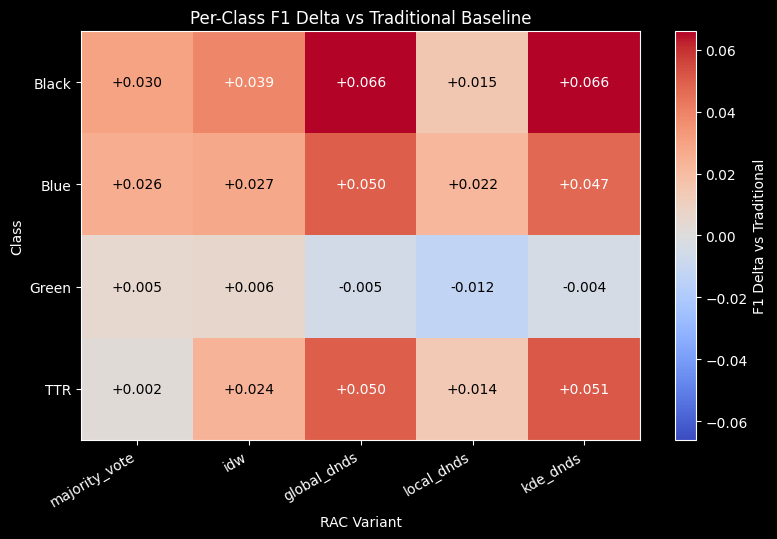
\includegraphics[width=\linewidth,height=0.58\textheight,keepaspectratio]{images/per_class_f1_delta.png}
    \\[-2pt]
    {\scriptsize Per-class F1 delta (RAC vs traditional)}
  \end{column}
  \begin{column}{0.5\textwidth}
    \centering
    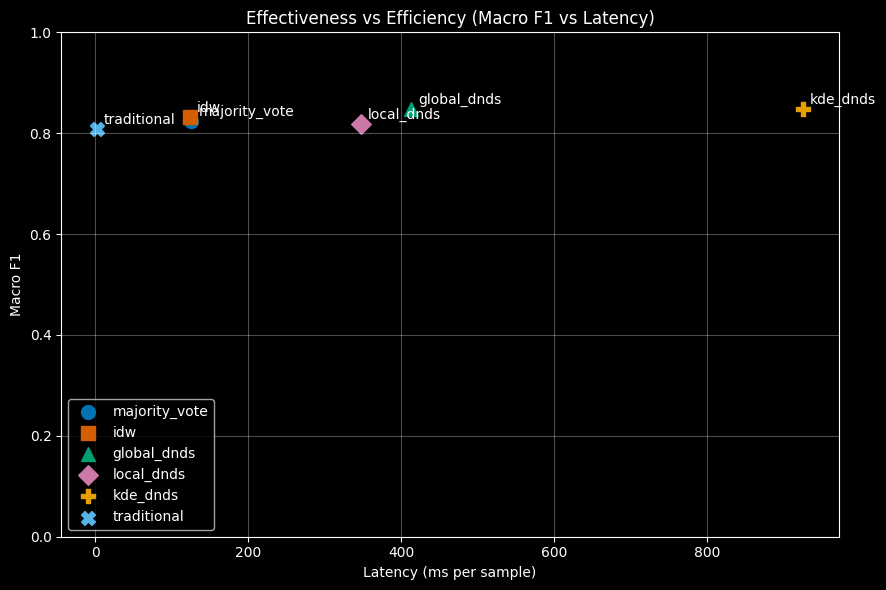
\includegraphics[width=\linewidth,height=0.58\textheight,keepaspectratio]{images/effectiveness_vs_efficiency.png}
    \\[-2pt]
    {\scriptsize Effectiveness vs efficiency frontier}
  \end{column}
\end{columns}
\end{frame}

\begin{frame}{Per-Class Improvements and Efficiency Trade-off: Takeaways}
\begin{itemize}
  \item RAC improves Macro-F1, but costs latency \cite{li2024kra}.
  \item Green can be over-penalized due to compact clusters \cite{yan2009studies}.
\end{itemize}
\end{frame}

\begin{frame}{Robustness Under Imbalance: All Classes}
\centering
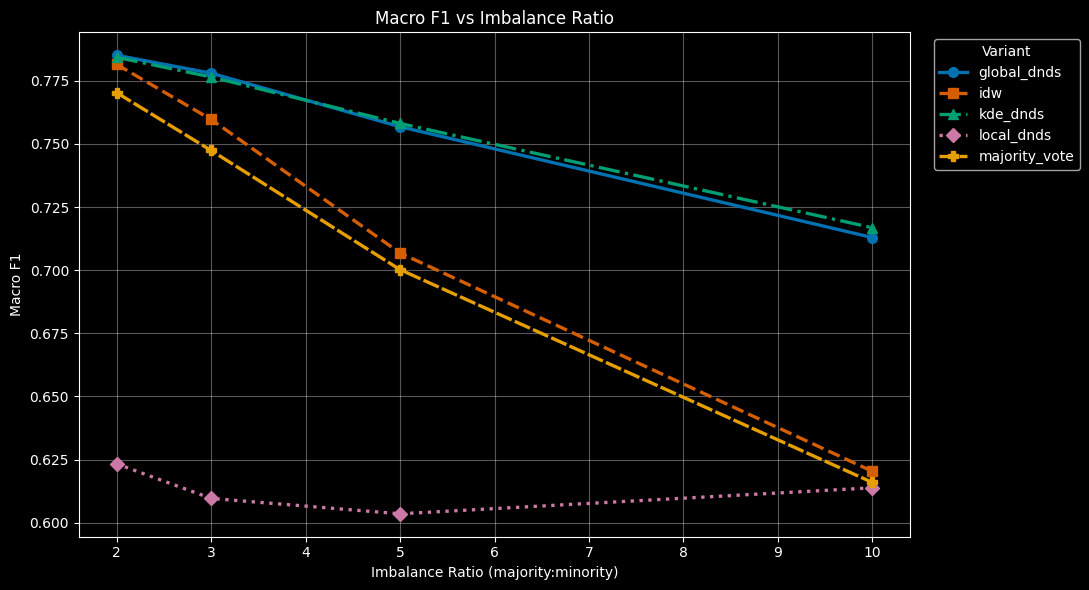
\includegraphics[width=0.92\linewidth,height=0.72\textheight,keepaspectratio]{images/f1_vs_imbalance.png}
\\[-2pt]
{\scriptsize All classes: F1 vs imbalance ratio}
\end{frame}

\begin{frame}{Robustness Under Imbalance: Minority Classes}
\centering
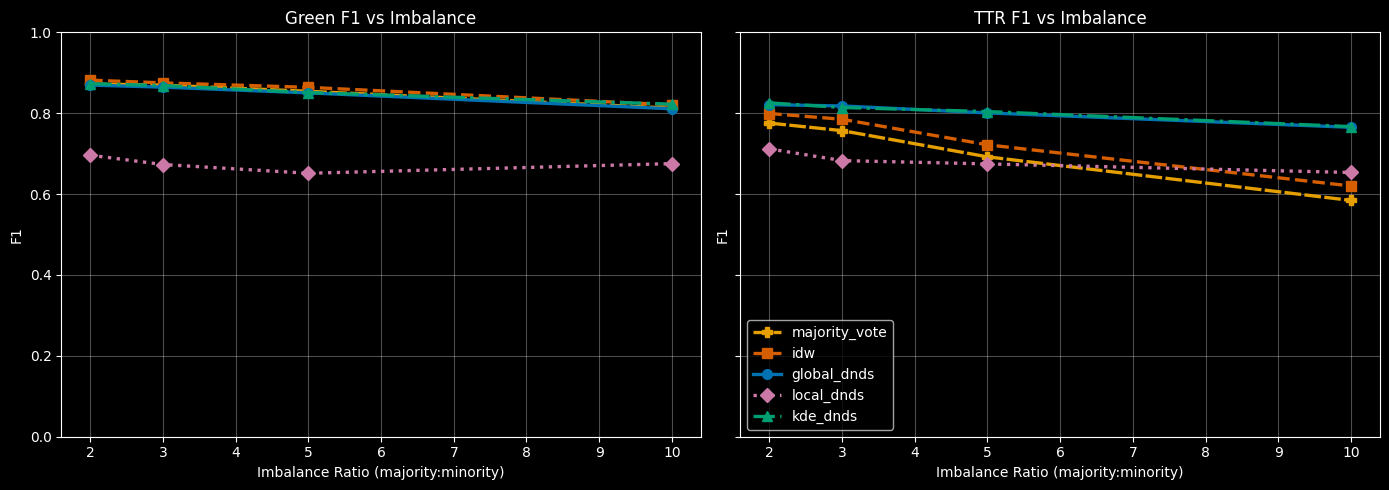
\includegraphics[width=0.92\linewidth,height=0.72\textheight,keepaspectratio]{images/f1_vs_minority-imbalance.png}
\\[-2pt]
{\scriptsize Minority classes (Green, TTR)}
\end{frame}

\begin{frame}{Robustness Under Imbalance: Takeaways}
\begin{itemize}
  \item Global and KDE DNDS degrade more gracefully under skew \cite{long2022retrieval,lakatos2025investigating}.
  \item KDE DNDS retains minority-class F1 slightly better.
\end{itemize}
\end{frame}

\begin{frame}{Continual Learning with Growing Database}
\begin{columns}[T]
  \begin{column}{0.56\textwidth}
    \centering
    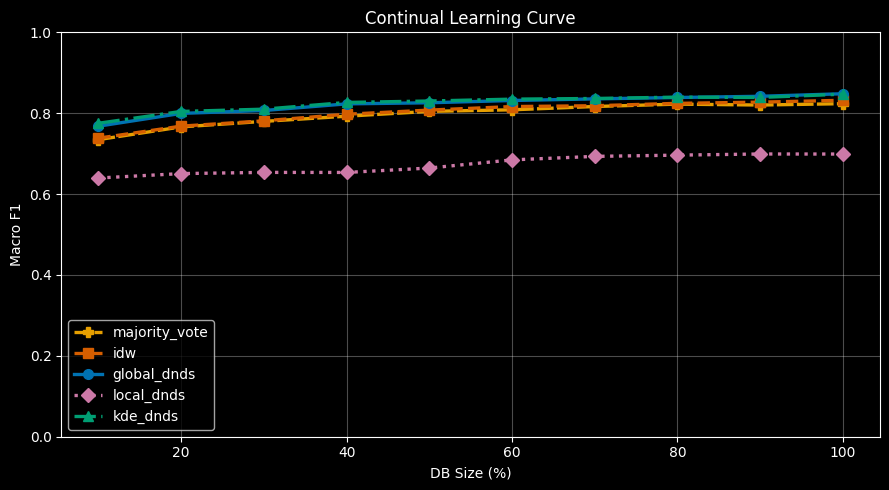
\includegraphics[width=\linewidth]{images/continual_learning.png}
  \end{column}
  \begin{column}{0.44\textwidth}
    \small
    \begin{itemize}
      \item All RAC variants improve as DB size increases.
      \item New data is usable immediately after insertion.
      \item Suitable for incremental deployment.
      \item Retrieval-augmented pipelines naturally benefit from richer neighbor pools \cite{li2024kra}.
    \end{itemize}
  \end{column}
\end{columns}
\end{frame}

\section{Discussion and Conclusion}
\begin{frame}{Discussion: Strengths and Limitations}
\textbf{Strengths}
\begin{itemize}
  \item Improves Macro-F1 without heavy end-to-end retraining.
  \item More robust than traditional fusion under imbalance \cite{long2022retrieval,lakatos2025investigating}.
\end{itemize}

\textbf{Limitations}
\begin{itemize}
  \item Higher inference latency from retrieval/scoring.
  \item Local DNDS is sensitive to $K_{density}$.
  \item Ceiling depends on embedding quality \cite{abimbola2026open,islam2026learning,li2025iris}.
\end{itemize}
\end{frame}

\begin{frame}{Conclusion}
\begin{itemize}
  \item RAC is a strong alternative to supervised multimodal fusion \cite{li2024kra,lakatos2025investigating}.
  \item \textbf{Global DNDS}: best overall on this dataset.
  \item \textbf{KDE DNDS}: better retention under severe skew.
  \item Traditional models remain best for strict low latency.
\end{itemize}

\vspace{8pt}
\centering
\textbf{Takeaway:} Effectiveness vs efficiency should be selected by deployment constraints, not accuracy alone.
\end{frame}

\begin{frame}[allowframebreaks]{References}
\scriptsize
\bibliographystyle{IEEEbib}
\bibliography{strings,refs}
\end{frame}

\end{document}
